\section{The ObFS File System:\\ Design \& Implementation}
\label{sec:obfs}
ObFS is based on the following principles:

1. Metadata is designed to be used in memory, not from storage.
Files are maps from extents within the file to extents within objects, and directories are maps from names to inode numbers and ancillary information.
Metadata objects are serialized into checkpoints and may then be flushed from memory and demand-loaded later, but the metadata serialization format is not designed to be mutable.

2. Data and metadata is persisted in a stream of objects tagged with sequence numbers as numeric prefixes, allowing efficient internal representation of object names.
Each object encodes a consecutive sequence of file system operations, allowing a consistent prefix to be recovered after failure even if multiple object writes are in progress at the time of failure.

3. Files, directories, and other file system objects (symlinks, special files) are identified by inode number.
These numbers are opaque identifiers and do not identify location, but instead are assigned from an incrementing counter.

4. Each object contains a logical journal of individual file system operations, described below, plus a data region containing the data for write operations in the journal.

\begin{figure}
\begin{framed}
{\footnotesize 
\begin{verbatim}
object "vdisk.0000":
  INODE num=1 mode=S_DIR|0777, size=0, uid/gid, timestamp
  CREATE parent=1 inum=2 name="file.txt"
  INODE num=2  mode=S_REG|0777, uid/gid, size=0, timestamp
  DATA 11 offset=0 dataptr=0 len=15 newsize=15
  --
  this is a test\n
\end{verbatim} }
\end{framed}

  \caption{ A trivial ObFS file system. \rm The root directory is inode 1; it contains a single file, ``file.txt'', with a 15-byte write starting at offset 0 in the object data segment.} 
  %(S\_REG is the POSIX mode flag for a ``regular'' file)}
  \label{figure:journal1}
\end{figure}

\begin{figure}
\begin{framed}
 {\footnotesize
\begin{verbatim}
object "vdisk.0001":
  CREATE parent=1 inum=3 name="dir1"
  INODE num=3 mode=S_DIR|0777, uid/gid, size=0, timestamp
  DATA num=2 offset=15 dataptr=0 len=15 newsize=40
  --
  this is another test\n
\end{verbatim} }
\end{framed}
  \caption{Second data object. \rm Creates subdirectory \texttt{/dir1} and adds 15 bytes to \texttt{/file.txt}.}
  \label{figure:journal2}
\end{figure}


\begin{figure}
\centering
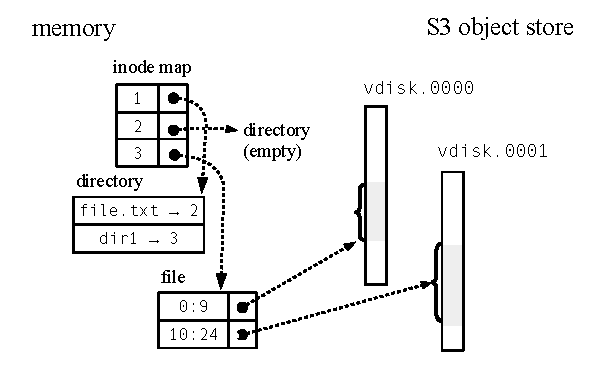
\includegraphics[width=0.95\columnwidth]{figs/obfs.pdf}
\caption{Relationship of in-memory structures and S3 objects for file system shown in Figures \ref{figure:journal1} and \ref{figure:journal2}.}
\label{figure:picture}
\end{figure}

\subsection{Logical Journal Format}

A trivial example of an ObFS file system may be seen in Figure~\ref{figure:journal1}.
It contains a journal of the following operations:
\begin{itemize}[nosep]
\item Modify root directory properties (inode 1) to set permissions, UID/GID, and timestamp
\item Create an entry for a new file, \texttt{/file.txt} in the root directory
\item Set inode properties for the file
\item Write 15 bytes to the file
\end{itemize}

At mount time the log will be replayed; when complete the root directory will have a single entry [\texttt{"file.txt"} $\rightarrow$ 2], and the file identified as inode 2 will have a single extent in its map, with offsets $[0\ldots 14]$ mapped to offset 0 in the data section of object 0.
In Figure~\ref{figure:journal2} we see the second object in the stream, journaling the creation of an empty directory (\texttt{/dir1}) and the write of 15 more bytes to \texttt{/file.txt}; again these will be reflected in in-memory data structures after journal recovery during the mount process.

\begin{table}
  \begin{tabular}{l|l}
    Operation & \rule{4em}{0pt} arguments \\
    \hline
    INODE & inum, mode, uid/gid, rdev, mtime \\
    CREATE & parent inum, inum, name \\
    RENAME & inum, parent inum1, inum2, name1, name2 \\
    TRUNC & inum, new size\\
    DELETE & parent inum, inum, name \\
    SYMLINK & inum, target\\
    DATA & inum, file offset/len, obj offset, new file size\\
    \hline
  \end{tabular} \vspace{0.5\baselineskip}
  \caption{ObFS journal entry types}
  \label{table:journal}
\end{table}

The full list of seven journal entry types may be seen in Table~\ref{table:journal}.
We believe that they are sufficient for basic POSIX file system functionality, although our implementation has taken some liberties with timestamps (we assume \texttt{noatime} mounts) and we have not yet implemented reference counting for hard links in either the in-memory or serialized metadata formats.

Figures~\ref{figure:journal1} and \ref{figure:journal2} show back-end storage objects which are ridiculously small, for illustrative purposes.
In practice objects would be written when either (a) a default size has been reached (e.g. 8-16\,MiB), (b) an idle timeout has passed (e.g. 1s), or (c) a synchronizing operation (\texttt{fsync}, etc.) is performed.
The file system may be operated in an unsafe mode by either ignoring synchronizing operations entirely, in which case failure may cause data and operation loss but will not result in an inconsistent file system, or by logging to local high-speed storage, in which case synchronized data may be lost in the case of catastrophic failures.

\subsection{In-memory metadata}
Although in-memory data structures for a file system may be considered implementation details rather than architecture, their functionality is central to the architecture of ObFS.
Our description of these structures is provided in order to explain this functionality in a straightforward fashion, rather than to constrain implementation\footnote{For instance, in a proper in-kernel VFS implementation the structures described would no doubt be ``absorbed'' into existing kernel data structures.}.

ObFS supports the standard UNIX/POSIX file system objects: files, directories, symbolic links, and various classes of special files (e.g. character devices) with no file system functionality.
All objects (in the OO sense) have basic metadata such as uid/gid and timestamps; with the addition of a device number this is sufficient for the special file types.
This object is extended with the following information for the remaining types:
\begin{itemize}[nosep]
\item \textbf{Symbolic link:} a single string, the link target.
\item \textbf{Directory:} a map from strings (i.e. names) to integer inode numbers.
\item \textbf{File:} a byte-granularity interval map from offset ranges within the file to (object, offset) pairs indicating the location of the data in an S3 object\footnote{We explicitly call these ``S3 objects'' here to differentiate from in-memory objects, however other S3-like services providing named objects may of course be used.} from storage objects; however , with S3 objects identified by their integer sequence number.
\end{itemize}

Finally an inode table is used to map inode numbers to objects; path traversal thus iterates between accesses to this table and to individual directories.

\subsection{Checkpoints}

If ObFS were to do nothing but log operations to storage then mounting a file system would soon become unwieldy, requiring the playback of all operations performed on the file system to date.
To avoid this we periodically checkpoint metadata to storage so that the file system may be mounted by locating the most recent checkpoint, loading that into memory, and then rolling the journal forward from that point.
Note that a clean unmount will perform a checkpoint after all writes are complete, eliminating any recover overhead at mount time.

As the file system grows, the memory requirements for in-memory metadata may grow excessive.
This may be addressed by demand-loading metadata from the most recent checkpoint, and evicting unmodified metadata objects from memory when necessary.
This requires a mechanism to map an inode number to its location in the checkpoint: the two obvious possibilities are (a) a mapping table in the checkpoint, or (b) appending the information to directory entries.
Our current design stores an inode number to location map in the checkpoint, in part because this mapping is needed during garbage collection, when the identity of the parent directory may not be known.
We expect to revisit this decision as we gain experience with larger file systems, as performance may suffer if this table grows too large to be held in memory.

With further growth of a file system the overhead of writing checkpoints will increase.
If a fixed checkpoint interval is maintained, then metadata write overhead will go up as the ratio of modified to total metadata shrinks.
However, if the checkpoint interval is allowed to expand proportionally to reduce this overhead, mount time will suffer.

This may be addressed by keeping multiple partial snapshots.
Rather than implementing a complex garbage collection mechanism we use a simple FIFO method, keeping the last N checkpoints and copying any un-replicated data from the oldest checkpoint when we make a new one.
The need to keep separate inode maps for each snapshot limits the number of snapshots which may be maintained in practice, and alternate methods may be needed to support volumes of more than a few tens of millions of files.

\subsection{Garbage Collection}

ObFS has been tested with a simple Greedy cleaning algorithm, selecting the least-utilized objects, reading and re-writing any remaining live data before object deletion.
This is known to be optimal for uniform memoryless workloads~\cite{yang_optimality_2015}, but to perform poorly when workloads are skewed or correlated~\cite{desnoyers_analytic_2014}. 
We therefore include several well-known techniques which greatly improve its performance on realistic workloads:

\textbf{Dual write frontiers:}~\cite{lin_dual_2012} In realistic workloads, data which has survived long enough to be copied during garbage collection has a longer expected time-to-live than new writes.
  ObFS garbage collection output is written into separate objects, implicitly performing hot/cold data segregation.

\textbf{Write coalescing:} The hottest data items will be overwritten before an object is written to storage.
  By merging data and metadata in an object before it is written out, this space may be reclaimed without any copying, or even writing it in the first place\footnote{This is not yet implemented in our prototype.}.

\textbf{Hysteresis-based batching:} Optimal cleaning of skewed workloads requires allowing blocks containing hot data to ``age'' to lower utilizations than those containing cold data~\cite{desnoyers_analytic_2014}.
  To do this optimally requires extensive bookkeeping; however in practice the simple hysteresis mechanism we use achieves most of its benefits, deferring cleaning until a low-water mark is reached, then cleaning until a high-water mark is reached.

To identify live data we read the DATA records from the object header, and for each check that the current extent map still refers to the same location.
If the relevant inode is in memory it may be looked up directly; if not, the inode location map is used to demand-load it.
Although not implemented in our current prototype, we plan to segregate metadata loaded for garbage collection and free it at the end of the cycle.

Finally we note that ObFS objects contain metadata such as directory and inode information (e.g. CREATE and INODE records) as well as data.
Garbage collection must therefore either (a) only consider objects for deletion which are older than the most recent full checkpoint, or (b) create a new checkpoint before deletion.
Our current prototype chooses option (b), checkpointing metadata before beginning a garbage collection cycle.

\subsection{Additional features}
We are extending ObFS to support snapshots, clones of a base file system image, and "native overlay"---a form of clone based on multiple parent file systems.
We describe these briefly due to space limitations.

\noindent \textbf{Cloning:} The object stream for a cloned volume looks almost exactly like that for a simple ObFS file system, with objects older than a certain sequence number belonging to the base image, and later objects belonging to the clone, using a different prefix for object names.

\noindent \textbf{Snapshots:} A snapshot is just a specific object in the stream and its predecessors.
Garbage collection continues in the presence of snapshots; however objects containing data referenced by snapshots are not deleted until those snapshots have been removed.

\noindent \textbf{Overlay:} This is performed via an ordered merge of the metadata from several underlying file systems\footnote{This involves translating inode numbers and object sequence numbers; lack of space prohibits a full explanation.}, which may then be written as the initial checkpoint of the merged volume.
Although this is a heavier-weight process than union mount, the resulting file system will operate at native speed.

%\cite{10.1109/SMARTCOMP.2014.7043841}
